% =====================================================================
% Snippet: bar-chart.tex
% =====================================================================
% USAGE: Benchmark bar chart with N bars, value labels, and grid.
% Copy tikzpicture content (lines marked %% COPY-START / END) into your
% figure.tex, then replace:
%   - data list: \def\bardata{...} — comma-separated "name/value"
%   - max_val: y-axis max (default 100, for percentages)
%   - title: chart title
%   - origin_x, origin_y: anchor position
%   - bar_color: highlight color (default acaBlueLine)
% =====================================================================

\documentclass[tikz,border=10pt]{standalone}
\usepackage{xcolor,tikz}
\usetikzlibrary{positioning,calc}

\definecolor{acaBlueLine}{HTML}{3060A8}
\definecolor{acaBlueFill}{HTML}{6890C8}
\definecolor{acaGreyLine}{HTML}{606060}

\begin{document}
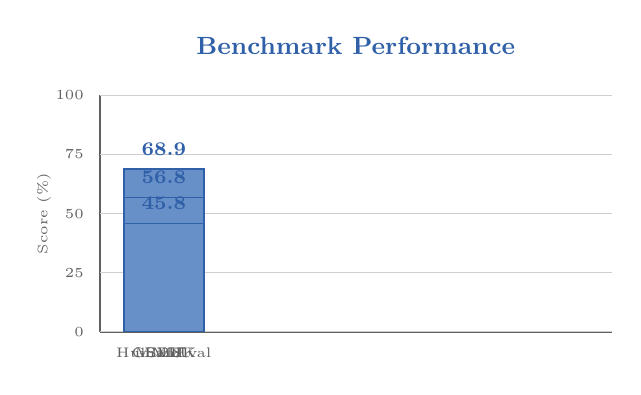
\begin{tikzpicture}

%% COPY-START =========================================================

% --- PARAMETERS ---
\def\bardata{MMLU/68.9, HumanEval/29.9, GSM8K/56.8, BBH/45.8}
\def\maxval{100}            % y-axis max
\def\chartW{6.5}            % chart width in cm
\def\chartH{3.0}            % chart height in cm
\def\xO{0}                  % origin x
\def\yO{0}                  % origin y
\def\barColor{acaBlueFill}
\def\barEdge{acaBlueLine}

% --- COUNT BARS ---
\pgfmathsetmacro\nbars{0}
\foreach \name/\val in \bardata {\xdef\nbars{\nbars+1}}
\pgfmathsetmacro\nbars{\nbars}
\pgfmathsetmacro\barW{\chartW / (\nbars * 1.6)}  % auto bar width
\pgfmathsetmacro\barGap{\chartW / \nbars}        % spacing between centers

% --- AXES ---
\draw[acaGreyLine, line width=0.6pt]
  (\xO, \yO) -- (\xO + \chartW, \yO);                % x-axis
\draw[acaGreyLine, line width=0.6pt]
  (\xO, \yO) -- (\xO, \yO + \chartH);                % y-axis

% --- Y-AXIS GRIDLINES + TICK LABELS ---
\foreach \pct in {0, 25, 50, 75, 100} {
  \pgfmathsetmacro\ypos{\yO + \chartH * \pct / \maxval}
  \draw[acaGreyLine!30, line width=0.3pt]
    (\xO, \ypos) -- (\xO + \chartW, \ypos);
  \node[anchor=east, font=\tiny, color=acaGreyLine]
    at (\xO - 0.08, \ypos) {\pct};
}
\node[anchor=south, font=\tiny, rotate=90, color=acaGreyLine]
  at (\xO - 0.5, \yO + \chartH/2) {Score (\%)};

% --- BARS ---
\pgfmathsetmacro\idx{0}
\foreach \name/\val in \bardata {
  \pgfmathsetmacro\idx{\idx+1}
  \pgfmathsetmacro\cx{\xO + \idx * \barGap - \barGap/2}
  \pgfmathsetmacro\bh{\chartH * \val / \maxval}
  % bar
  \fill[\barColor]
    (\cx - \barW/2, \yO) rectangle (\cx + \barW/2, \yO + \bh);
  \draw[\barEdge, line width=0.5pt]
    (\cx - \barW/2, \yO) rectangle (\cx + \barW/2, \yO + \bh);
  % value label on top
  \node[anchor=south, font=\scriptsize\bfseries, color=\barEdge]
    at (\cx, \yO + \bh + 0.05) {\val};
  % x-axis label
  \node[anchor=north, font=\tiny, align=center, color=acaGreyLine]
    at (\cx, \yO - 0.08) {\name};
}

% --- TITLE ---
\node[anchor=south, font=\small\bfseries, color=\barEdge]
  at (\xO + \chartW/2, \yO + \chartH + 0.4) {Benchmark Performance};

%% COPY-END ===========================================================

\end{tikzpicture}
\end{document}
